% ====================================================================
% VİZE RAPOR ŞABLONU – Türk Masalları Derlemesi Web Sayfası
% --------------------------------------------------------------------
% DERLEME: Overleaf'te Menu > Compiler > XeLaTeX (pdfLaTeX de çalışır).
%
% KURALLAR (şablonu kullanmadan önce okuyun):
%  1. Bölüm başlıklarını SİLMEYİN ve sırasını DEĞİŞTİRMEYİN.
%  2. [KÖŞELİ PARANTEZ] içindeki ve gri renkli açıklama metinlerini
%     kendi bilgilerinizle değiştirin; açıklama metinlerini silin.
%  3. MEBİS'e YALNIZCA bu raporun PDF'ini yükleyin.
%     ZIP ve HTML dosyası YÜKLEMEYİN. Tüm kontroller GitHub'dan yapılır.
%  4. Kapaktaki GitHub ve YouTube bağlantıları doğru ve tıklanabilir
%     olmalıdır. Teslimden önce PDF'teki bağlantılara tıklayıp deneyin.
%  5. Haftalık katkı tablosundaki görseller için resim dosyalarını
%     (hafta1.png, hafta2.png, ...) Overleaf projesine yükleyin.
%     Dosya adlarında boşluk ve Türkçe karakter kullanmayın.
%     Resim yoksa tabloda "görsel ekleyin" kutusu görünür.
%  6. Yapay zekâ kullandıysanız Bölüm 5'i doldurun.
% ====================================================================
\documentclass[12pt,a4paper]{article}

\usepackage{iftex}
\ifPDFTeX
  \usepackage[T1]{fontenc}
  \usepackage[utf8]{inputenc}
\else
  \usepackage{fontspec}
\fi
\usepackage[turkish]{babel}
\usepackage[margin=2.4cm]{geometry}
\usepackage{setspace}
\usepackage{graphicx}
\usepackage{booktabs}
\usepackage{longtable}
\usepackage{array}
\usepackage{colortbl}
\usepackage{xcolor}
\usepackage{enumitem}
\usepackage{listings}
\usepackage{amssymb}
\usepackage{caption}
\usepackage{fancyhdr}
\usepackage{hyperref}

\onehalfspacing
\setlength{\parindent}{0pt}
\setlength{\parskip}{6pt}
\setlist{itemsep=2pt, topsep=4pt}
\hypersetup{colorlinks=true, linkcolor=blue!50!black, urlcolor=blue!50!black}

\definecolor{ana}{HTML}{14325C}
\definecolor{acik}{HTML}{EEF2F8}

\lstset{basicstyle=\ttfamily\small, backgroundcolor=\color{acik},
  frame=single, rulecolor=\color{ana}, breaklines=true,
  columns=fullflexible, keepspaces=true, showstringspaces=false}

\pagestyle{fancy}
\fancyhf{}
\fancyhead[L]{Bir Varmış Bir Yokmuş}
\fancyhead[R]{Vize Raporu}
\fancyfoot[C]{\thepage}

% ---------- Yardımcı komutlar ----------
% Gri açıklama metni (silinecek yönergeler için)
\newcommand{\aciklama}[1]{{\color{gray}\itshape (#1)}}

% Haftalık tablo görseli: dosya yoksa "görsel ekleyin" kutusu çıkar
\newcommand{\haftagorsel}[1]{%
  \IfFileExists{#1}{%
    \includegraphics[width=\linewidth,height=4.2cm,keepaspectratio]{#1}%
  }{%
    \fbox{\parbox[c][2.6cm][c]{\dimexpr\linewidth-2\fboxsep-2\fboxrule\relax}{%
      \centering\small\color{gray} Ekran görüntüsü / görsel ekleyin\\ \texttt{#1}}}%
  }%
}
% Haftalık katılım kutuları (işaretlemek için $\square$ yerine $\boxtimes$ yazın)
\newcommand{\katilimkutulari}{\par\vspace{3pt}\small $\square$ Ders içinde katılım sergiledim\par $\square$ Telafi yaptım}

% Ek görsel: dosya yoksa hiçbir şey göstermez
\newcommand{\haftaek}[1]{%
  \IfFileExists{#1}{\\[4pt]\includegraphics[width=\linewidth,height=4.2cm,keepaspectratio]{#1}}{}%
}

% ---------- Kapak bilgileri ----------
\newcommand{\universite}{İstanbul Medipol Üniversitesi / Görsel İletişim Tasarımı}
\newcommand{\dersadi}{Programlamaya Giriş}
\newcommand{\hocaadi}{Meral Şentürk}
\newcommand{\ogrenciadi}{İlayda Akgün}
\newcommand{\ogrencino}{86230049}
\newcommand{\projeadi}{Bir Varmış Bir Yokmuş}
% Bağlantıları tam adres olarak yazın (https:// ile başlayarak)
\newcommand{\githublink}{\url{https://github.com/iakgn649/bir---varmis---bir---yokmus}}
\newcommand{\youtubelink}{\url{https://youtu.be/GbCG_Iaj450}}

\begin{document}

% ====================================================================
% KAPAK
% ====================================================================
\begin{titlepage}
\centering
\vspace*{1cm}
{\large \universite \par}
\vspace{1.8cm}
{\Huge\bfseries\color{ana} \projeadi \par}
\vspace{0.4cm}
{\Large Türk Masalları Derlemesi Web Sayfası \par}
{\large Vize Raporu \par}
\vspace{1.8cm}
{\large \textbf{Ders:} \dersadi \par}
{\large \textbf{Öğretim Üyesi:} \hocaadi \par}
\vspace{1.2cm}
{\large \textbf{Hazırlayan:} \ogrenciadi \par}
{\large \textbf{Öğrenci No:} \ogrencino \par}
\vspace{1.8cm}
\fbox{\parbox{0.88\linewidth}{\centering\vspace{6pt}
{\large\bfseries Proje Bağlantıları}\\[8pt]
\textbf{GitHub deposu:}\\ \githublink \\[8pt]
\textbf{YouTube sunum videosu:}\\ \youtubelink
\vspace{6pt}}}
\vfill
{\large \today \par}
\end{titlepage}

\tableofcontents
\newpage

% ====================================================================
\section{Giriş}
% ====================================================================
Bu projede, Türk halk anlatı geleneğinden seçtiğim sekiz masalı bir araya getiren bir web sayfası hazırladım. Projeye, masalların geleneksel başlangıcını hatırlatan “Bir Varmış Bir Yokmuş” adını verdim. Amacım, kullanıcıların istedikleri masala kolayca ulaşabildiği ve rahatça okuyabildiği bir arayüz oluşturmaktı. Sayfanın yapısını HTML, görünümünü CSS ve etkileşimlerini JavaScript ile hazırladım. Bütün kodları tek bir HTML dosyasında topladım ve sayfanın internet bağlantısı olmadan çalışmasını sağladım. Masal seçme, ada göre arama, rastgele masal açma, yazı boyutunu değiştirme ve gece modu özelliklerini ekledim. Bu raporda masal seçimlerini, tasarım kararlarını, kodların çalışma mantığını ve yaptığım kontrolleri açıklıyorum.



\subsection{Proje Özeti}
Bir Varmış Bir Yokmuş, sekiz Türk masalının kısaltılmış yeniden anlatımlarını içeren bir okuma sayfasıdır. Kullanıcılar listeden veya arama alanından masal seçebilir, rastgele bir masal açabilir ve okuma görünümünü ayarlayabilir. Sayfa, dar ekranlarda liste ve okuma alanını alt alta yerleştiren bir düzene sahiptir. Masal metinlerinin hazırlanmasında kaynaklardan ve ChatGPT desteğinden yararlanılmıştır.

\subsection{Gereksinimlerin Karşılanması}
\begin{center}
\rowcolors{2}{acik}{white}
\begin{tabular}{@{}p{8.2cm}c@{}}
\toprule
\rowcolor{ana}\textcolor{white}{\textbf{Gereksinim}} & \textcolor{white}{\textbf{Durum}} \\
\midrule
Masal sayısı 8--12 arasında (8 masal)         & $\boxtimes$ \\
Tek HTML dosyası                                    & $\boxtimes$ \\
Stil kodları içsel (\texttt{<style>} içinde)        & $\boxtimes$ \\
Betik kodları içsel (\texttt{<script>} içinde)      & $\boxtimes$ \\
İnternetsiz açılıp çalışıyor                        & $\boxtimes$ \\
JavaScript sayfada anlamlı bir işlev görüyor        & $\boxtimes$ \\
Masal metinleri kendi cümlelerimle yazıldı        & $\square$ \\
Masal metinleri kendi cümlelerimle yazıldı               & $\square$ \\
\bottomrule
\end{tabular}
\end{center}

% ====================================================================
\section{Masalların Seçimi}
% ====================================================================
Derleme için önceden belirlediğim sekiz Türk masalını kullandım. Bu masallar; iyilik, zekâ, cesaret, sevgi ve öğüt gibi farklı temaları bir araya getiriyor. Kaynak metinlerden yararlanılarak ChatGPT desteğiyle kısaltılmış yeniden anlatımlar hazırlandı. Yararlanılan internet sayfaları kaynakça bölümünde belirtilmiştir.

\begin{longtable}{@{}cp{4cm}p{3cm}p{5.4cm}@{}}
\toprule
\textbf{No} & \textbf{Masal} & \textbf{Tür} & \textbf{Seçilme nedeni} \\
\midrule
\endhead
1 & Öksüz Kız & Olağanüstü masal & İyilik ve yardımlaşma temasını işlemesi. \tabularnewline
2 & Üç Turunçlar & Olağanüstü masal & Yolculuk ve dönüşüm motiflerini içermesi. \tabularnewline
3 & Zümrüdüanka Kuşu & Olağanüstü masal & Cesaret ve iyiliğin karşılığını anlatması. \tabularnewline
4 & Keloğlan ve Padişahın Kızı & Keloğlan masalı & Zekâ ve hazırcevaplığı öne çıkarması. \tabularnewline
5 & Tuz Kadar Sevgi & Öğretici masal & Sevginin değerini anlatması. \tabularnewline
6 & Dört Öğüt & Öğretici masal & Düşünerek davranmanın önemini göstermesi. \tabularnewline
7 & Hüsnü Yusuf & Olağanüstü masal & İnsan ve kuş biçimine dönüşme motifini içermesi. \tabularnewline
8 & Keloğlan ve Altın Bülbül & Olağanüstü masal & Kararlılık ve kıskançlığı işlemesi. \tabularnewline

\end{longtable}

% ====================================================================
\section{Tasarım Kararları}
% ====================================================================
Sayfayı masal okumayı kolaylaştıracak sade bir düzende tasarladım. Renkleri, düğmeleri ve yazı düzenini denemeler yaparak belirledim. Masal listesini ve okuma alanını birbirinden ayırdım. Hazır web sitesi şablonu kullanmadım; kodları ChatGPT desteğiyle adım adım oluşturdum ve tasarım tercihlerime göre düzenledim.

\subsection{Konuya Uygunluk}
Bordo, krem ve altın tonlarını masal kitabını hatırlatan sıcak bir görünüm oluşturmak için seçtim. Georgia yazı tipinin kitap hissini desteklediğini düşündüm. Masal başlıklarına içerikleriyle ilişkili küçük simgeler ekledim. Büyük başlangıç harfi, numaralandırılmış masal listesi ve metin sonundaki işaretle bu görünümü tamamladım. Gece modunda dış zemini koyulaştırıp masal düğmelerini krem bırakarak okunabilir bir karşıtlık oluşturdum.

\subsection{Renk Paleti ve Yazı Tipi}
\begin{center}
\rowcolors{2}{acik}{white}
\begin{tabular}{@{}llp{6.4cm}@{}}
\toprule
\rowcolor{ana}\textcolor{white}{\textbf{Ad}} & \textcolor{white}{\textbf{Kod}} & \textcolor{white}{\textbf{Nerede / neden kullandınız?}} \\
\midrule

Bordo & \texttt{\#722F37} & Üst başlıkta ve seçilen masal düğmesinde vurgu oluşturmak için kullanıldı. \tabularnewline
Krem & \texttt{\#F6EFE3} & Sayfanın zemininde ve düğmelerde sıcak bir görünüm oluşturmak için kullanıldı. \tabularnewline
Altın tonu & \texttt{\#BC955C} & İnce çizgilerde ve süsleme detaylarında kullanıldı. \tabularnewline
Georgia & -- & Kitap hissini desteklemek ve metinleri rahat okutmak için seçildi. \tabularnewline
\bottomrule
\end{tabular}
\end{center}

\subsection{Okunabilirlik, Gezinme ve Duyarlı Tasarım}
\begin{itemize}
  \item \textbf{Okunabilirlik:} Georgia yazı tipini, rahat satır aralığını ve zeminle karşıtlık oluşturan metin renklerini kullandım. Kullanıcının metni kendisine göre ayarlayabilmesi için yazıyı büyütme ve küçültme düğmeleri ekledim.
  \item \textbf{Gezinme:} Kullanıcı sekiz masaldan birini listeden seçebilir veya arama alanına masal adını yazarak listeyi daraltabilir. Seçilen masalın düğmesi bordo renkte kalır. “Bana bir masal seç” düğmesiyle rastgele bir masal da açılabilir.
  \item \textbf{Duyarlı tasarım:} Geniş ekranda masal listesi solda, okuma alanı sağda yer alır. Ekran genişliği 700 piksel ve altına indiğinde bu alanlar alt alta geçer. Bu düzeni bilgisayarda tarayıcı penceresini daraltarak kontrol ettim.
  \item \textbf{Tutarlılık:} Başlıklarda, düğmelerde ve kenarlıklarda aynı renkleri ve yuvarlatılmış biçimleri kullandım. Masalları numaralandırdım ve başlıklarına küçük simgeler ekledim. Gündüz ve gece modlarında aynı yerleşimi korudum.
\end{itemize}

\subsection{Ekran Görüntüleri}
\shorthandoff{=}
\begin{figure}[htbp]
\centering
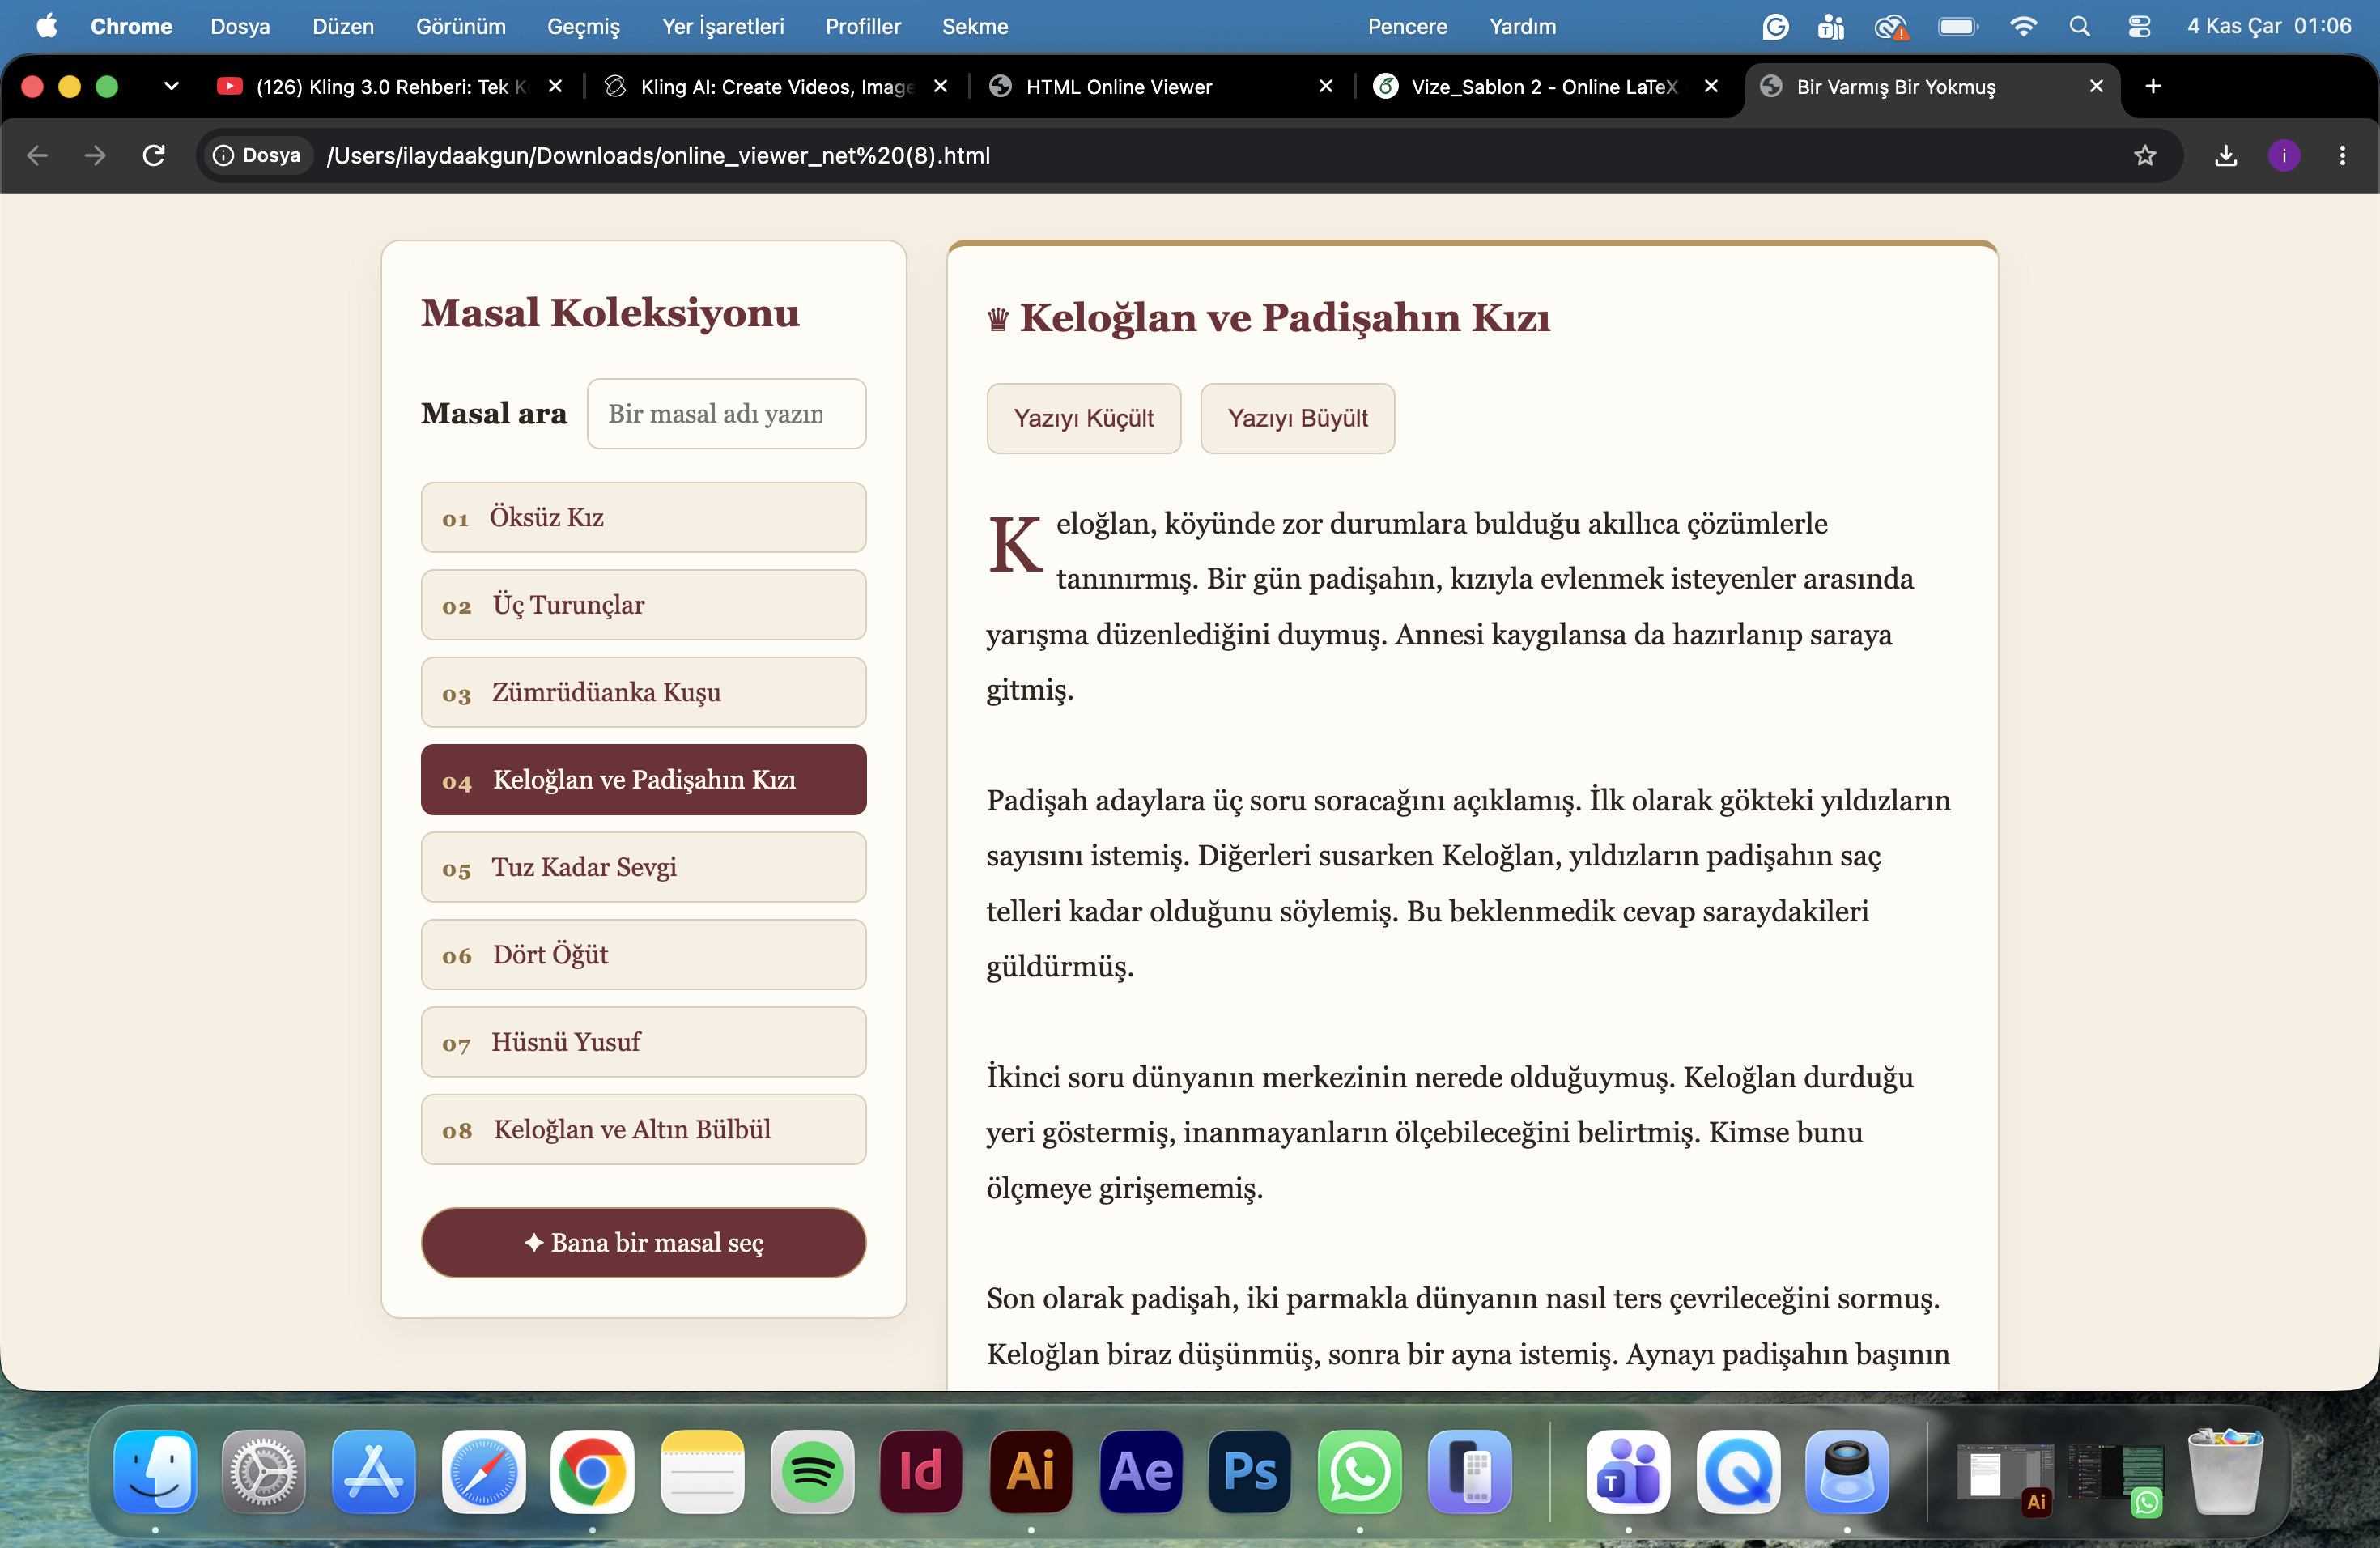
\includegraphics[height=7cm]{gunduz.png}

\caption{Web sayfasının gündüz modu görünümü}
\end{figure}

\begin{figure}[htbp]
\centering

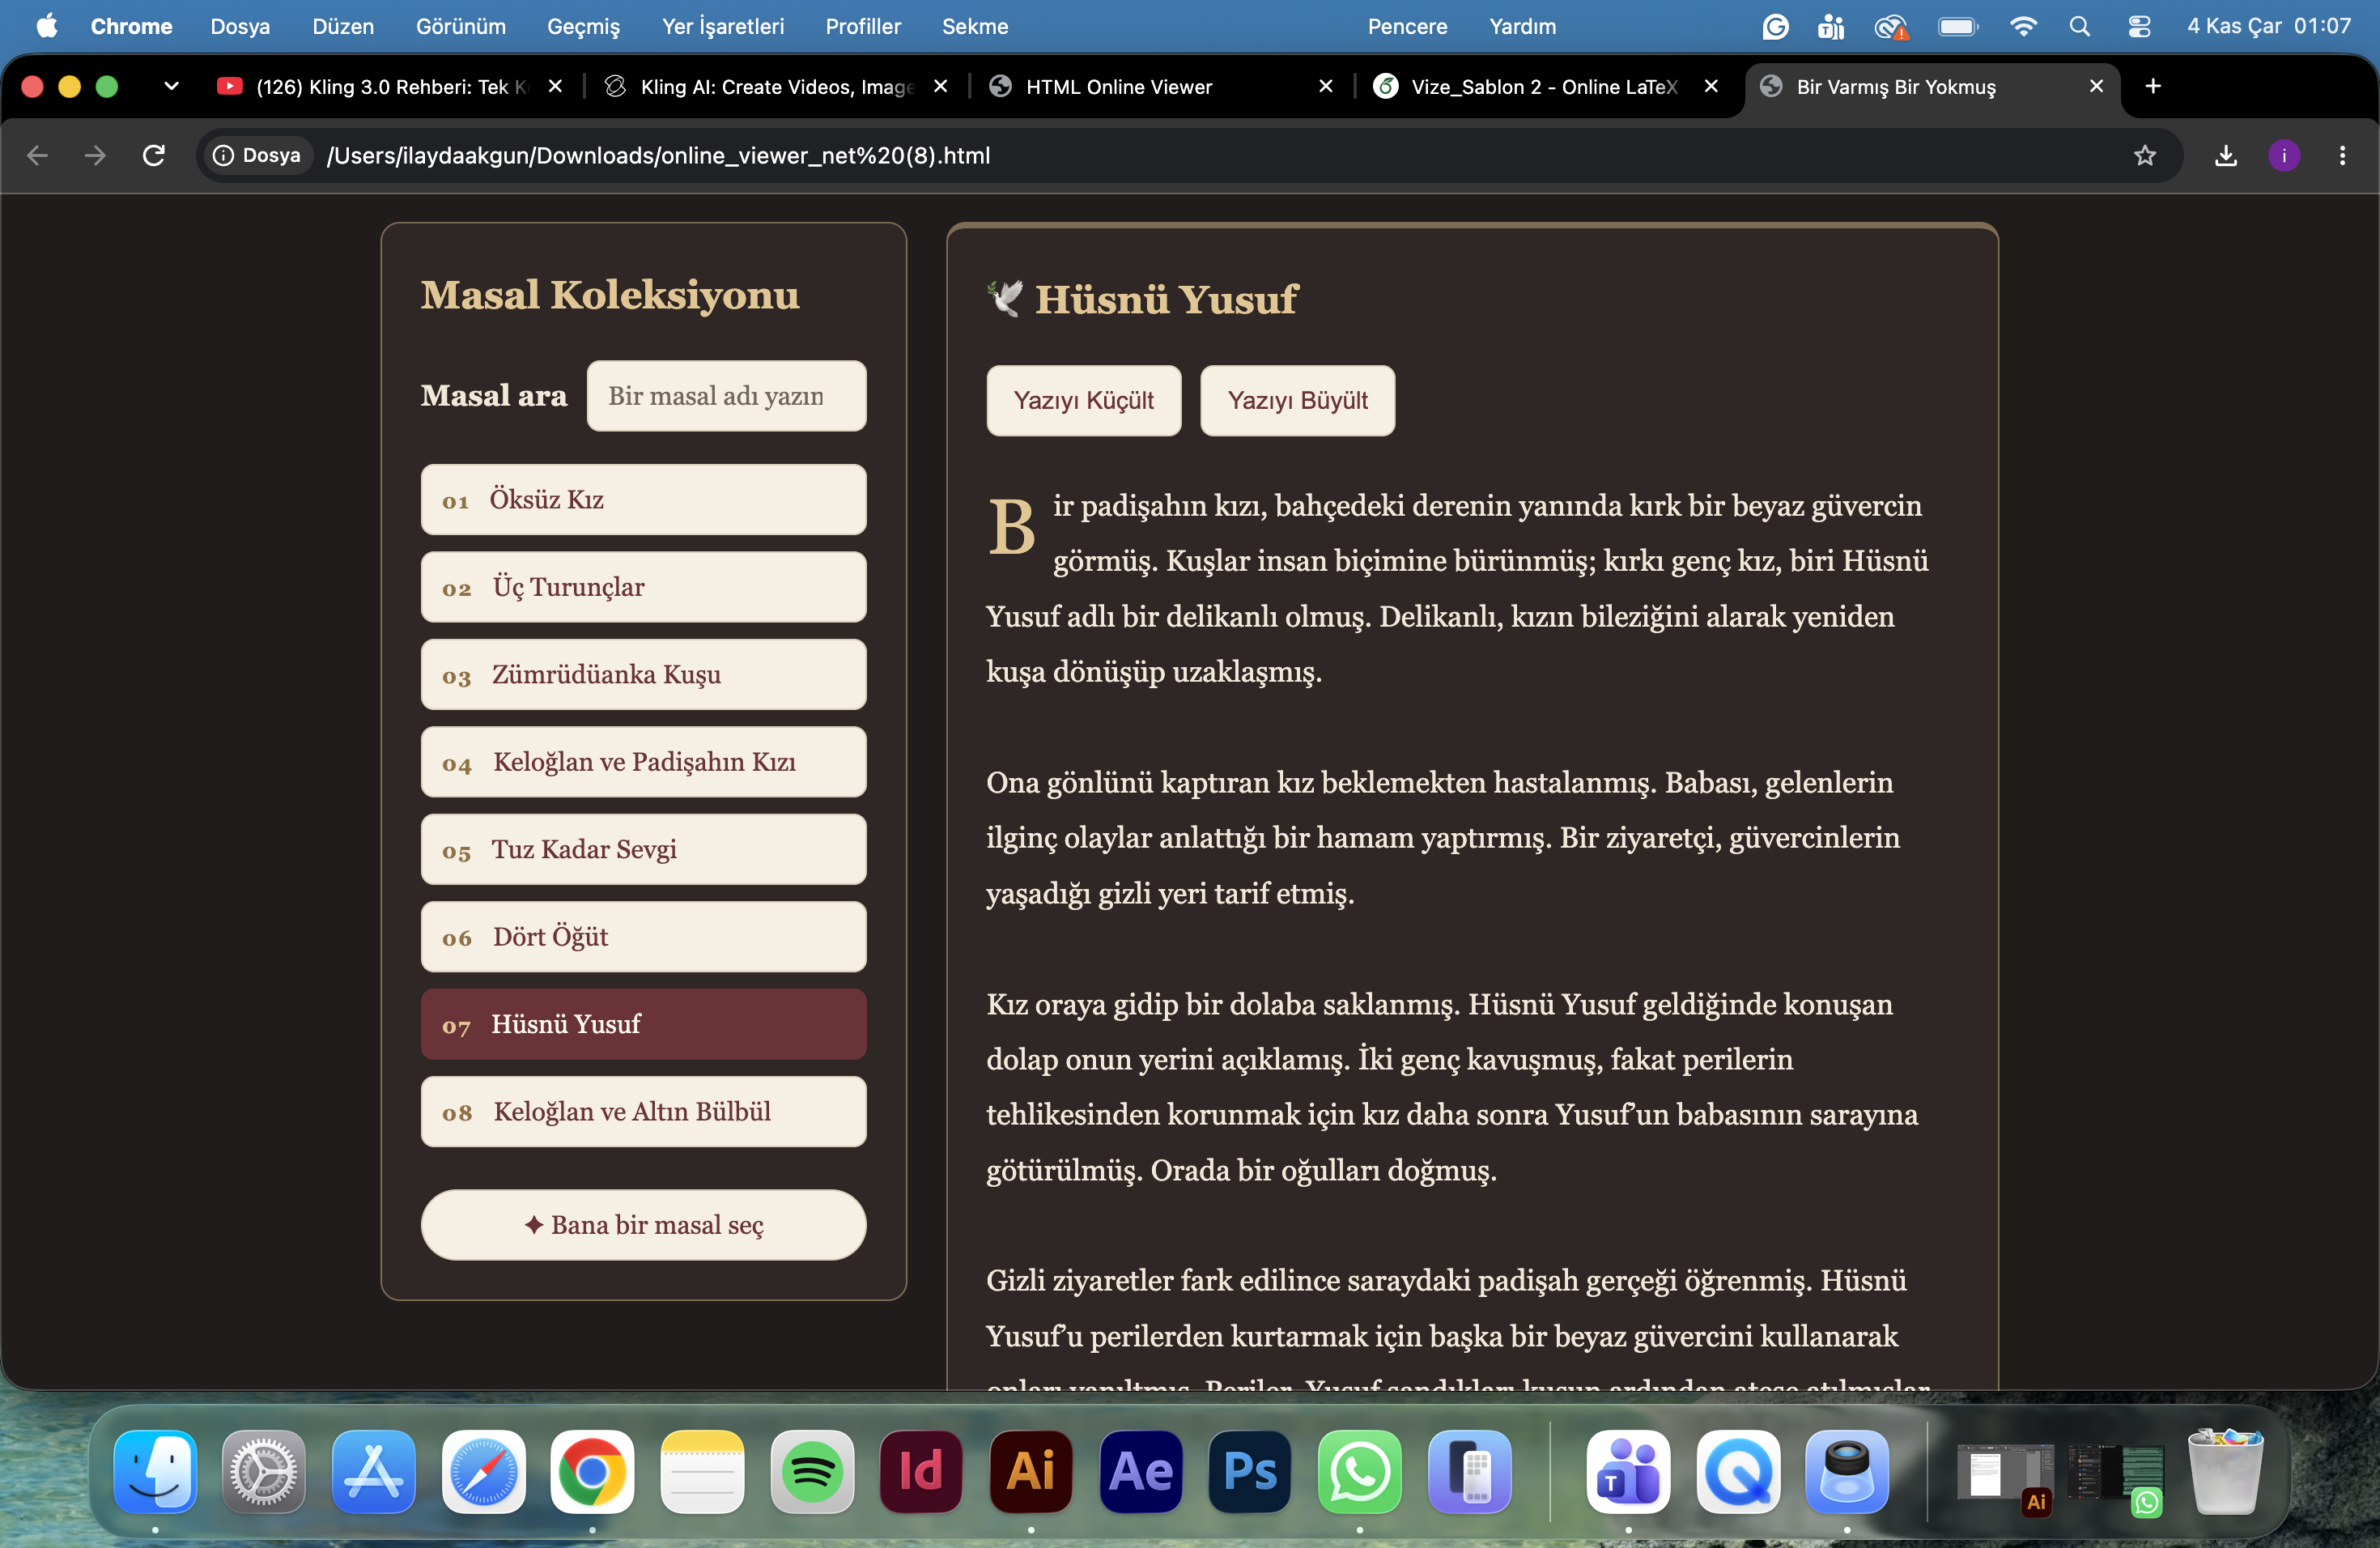
\includegraphics[height=7cm]{gece.png}
\caption{Web sayfasının gece modu görünümü}
\end{figure}

\clearpage
% \begin{figure}[h]
%   \centering
%   \includegraphics[width=0.9\textwidth]{ekran-masaustu.png}
%   \caption{Sayfanın bilgisayar görünümü}
% \end{figure}
% \begin{figure}[h]
%   \centering
%   \includegraphics[width=0.35\textwidth]{ekran-mobil.png}
%   \caption{Sayfanın telefon görünümü}
% \end{figure}

% ====================================================================
\section{Gerçekleştirme}
% ====================================================================
Web sayfasını tek bir HTML dosyası içinde hazırladım. HTML ile içerik alanlarını oluşturdum, CSS ile görünümü düzenledim ve JavaScript ile kullanıcı etkileşimlerini ekledim. Stil kodları style, JavaScript kodları ise script etiketlerinin içinde bulunuyor. Harici yazı tipi veya kütüphane kullanılmadığı için sayfa internet bağlantısı olmadan çalışabiliyor.

\subsection{HTML Yapısı}
Sayfanın üst bölümünde header etiketi içinde proje adı, kısa açıklama ve tema değiştirme düğmesi bulunuyor. main etiketi ana içeriği kapsıyor. section bölümünde arama alanı, nav içinde masal düğmeleri ve rastgele masal seçme düğmesi yer alıyor. article bölümünde seçilen masalın başlığı, yazı boyutu düğmeleri ve metni gösteriliyor. footer bölümünde derlemenin adı ve hazırlayan bilgisi bulunuyor. JavaScript’in ilgili alanları bulabilmesi için başlık, metin ve işlev düğmelerine id değerleri verdim.

\subsection{İçsel CSS}
CSS kodlarını HTML dosyasındaki style etiketi içinde tuttum. Ana yerleşimde grid kullanarak masal listesi ve okuma alanını iki sütuna ayırdım. Arama etiketi ile kutusunu yan yana yerleştirmek için flex kullandım. Ekran genişliği 700 piksel ve altına indiğinde düzenin tek sütuna geçmesini sağladım. Renkler, boşluklar, kenarlıklar ve düğmelerin görünümünü CSS ile düzenledim. Gece modu için body etiketine eklenen gece sınıfına bağlı farklı renk kuralları tanımladım

\begin{lstlisting}[caption={İçsel CSS'ten önemli bir bölüm}]
main {
display: grid;
grid-template-columns: 1fr 2fr;
gap: 24px;
}

@media (max-width: 700px) {
main {
grid-template-columns: 1fr;
}
}
\end{lstlisting}

\subsection{İçsel JavaScript}
JavaScript kodlarını HTML dosyasındaki script etiketi içinde tuttum. Masal düğmelerini querySelectorAll ile seçip her birine tıklama olayı ekledim. Tıklanan düğmenin adına göre if ve else if koşullarıyla ilgili masal metnini gösterdim. Seçilen düğmeye secili sınıfını ekleyerek renginin değişmesini sağladım. Arama alanı, yazılan ifadeyi masal adlarıyla karşılaştırıp eşleşmeyen düğmeleri gizliyor. Yazı boyutu düğmeleri metni 14 ile 30 piksel arasında ayarlıyor. Tema düğmesi body üzerindeki gece sınıfını değiştiriyor. Rastgele masal düğmesi ise rastgele bir sıra belirleyip ilgili masal düğmesini çalıştırıyor.

\begin{lstlisting}[caption={İçsel JavaScript'ten önemli bir bölüm}]
document.getElementById("buyut").addEventListener("click", function() {
if (yaziBoyutu < 30) {
yaziBoyutu = yaziBoyutu + 2;
metin.style.fontSize = yaziBoyutu + "px";
}
});
\end{lstlisting}

\subsection{Sayfanın Özellikleri}


% ====================================================================
\section{Yapay Zekâ Kullanımı}
% ====================================================================
Sayfada sekiz masalın kısaltılmış yeniden anlatımı bulunmaktadır. Kullanıcılar masal seçebilir, masal adına göre arama yapabilir ve rastgele bir masal açabilir. Yazı boyutu ayarlanabilir ve gündüz ile gece modu arasında geçiş yapılabilir. Seçilen masal renk değişimiyle belirtilir. Masal başlıklarında küçük simgeler, listede sıra numaraları bulunur. Sayfa tek HTML dosyası olarak internet bağlantısı olmadan çalışır.

\begin{longtable}{@{}p{2.6cm}p{3.6cm}p{4.2cm}p{3.4cm}@{}}
\toprule
\textbf{Araç} & \textbf{Ne için kullandınız?} & \textbf{İstem (prompt) özeti} & \textbf{Sayfada nerede?} \\
\midrule
\endhead
ChatGPT & HTML, CSS ve JavaScript desteği & Masal seçme, arama, yazı boyutu, tema ve rastgele seçim özelliklerini adım adım oluşturma ve hataları düzeltme. & Sayfanın yapısı, tasarımı ve etkileşimleri. \tabularnewline
ChatGPT & Metin desteği & Seçilen sekiz masalı belirtilen kaynaklara göre kısaltarak yeniden anlatma ve rapor taslağı hazırlama. & Masal metinleri ve rapor. \tabularnewline
\bottomrule
\end{longtable}

\subsection{Anladığım ve Kendim Yaptığım Kısımlar}
Masalları önceden belirledim. Kodları editöre adım adım ekledim ve her aşamada sayfanın görünümünü ve düğmelerini kontrol ettim. Bordo ve krem renklerini, gece modundaki açık renkli düğmeleri ve düğme adlarını kendi tercihlerime göre düzenlettim. Çalışmayan bölümleri ekran görüntüleri ve kod parçaları üzerinden inceleyerek destekle düzelttim. HTML’in içerik yapısını, CSS’in görünümü ve JavaScript’in etkileşimleri yönettiğini öğrendim.

% ====================================================================
\section{Haftalık Katkılar}
% ====================================================================


\begin{longtable}{@{}>{\raggedright\arraybackslash}p{1.7cm}%
                    >{\raggedright\arraybackslash}p{6.4cm}%
                    >{\centering\arraybackslash}p{6cm}@{}}
\toprule
\rowcolor{ana}\textcolor{white}{\textbf{Hafta}} & \textcolor{white}{\textbf{Yapılan çalışma}} & \textcolor{white}{\textbf{Görsel}} \\
\midrule
\endfirsthead
\toprule
\rowcolor{ana}\textcolor{white}{\textbf{Hafta}} & \textcolor{white}{\textbf{Yapılan çalışma}} & \textcolor{white}{\textbf{Görsel}} \\
\midrule
\endhead
\bottomrule
\endfoot

\textbf{1. hafta}\newline [16.09.2026] &
Harry Potter konulu bir web sayfası hazırladım. Başlık ve paragraf etiketlerini kullanarak içerikleri sayfaya yerleştirdim. Bu çalışmayı telafi kapsamında tamamladım.\newline \textbf{Commit:} Bu çalışma için GitHub commit kaydı bulunmuyor.\par \(\square\) Ders içinde katılım sergiledim
\par \(\boxtimes\) Telafi yaptım&
\vspace{0pt}\haftagorsel{hafta1.png}\haftaek{hafta1b.png} \\
\midrule
\textbf{2. hafta}\newline [23.09.2026] &
Harry Potter konulu web sayfasında konu listesini ve sayfa içi bağlantıları düzenledim. Yazar, Hogwarts ve karakterler gibi bölümleri başlıklarla ayırdım. Bu çalışmayı telafi kapsamında tamamladım.\newline \textbf{Commit:}Bu çalışma için GitHub commit kaydı bulunmuyor.\par \(\square\) Ders içinde katılım sergiledim \par \(\boxtimes\) Telafi yaptım&
\vspace{0pt}\haftagorsel{hafta2.png}\haftaek{hafta2b.png} \\
\midrule
\textbf{3. hafta}\newline [30.09.2026] &
Kullanıcının adını girebildiği bir selamlama uygulaması hazırladım. Düğmeye basıldığında girilen adla birlikte selamlama mesajı gösterilmesini sağladım. Ad alanı boş bırakıldığında uyarı veren bir kontrol kullandım. Bu çalışmayı telafi kapsamında tamamladım.\newline \textbf{Commit:} Bu çalışma için GitHub commit kaydı bulunmuyor.\par \(\square\) Ders içinde katılım sergiledim \par \(\boxtimes\) Telafi yaptım&
\vspace{0pt}\haftagorsel{hafta3.png}\haftaek{hafta3b.png} \\
\midrule
\textbf{4. hafta}\newline [07.10.2026] &
Sinema bileti sayısını artırıp azaltan bir sayaç uygulaması hazırladım. JavaScript ile düğmelere tıklanınca sayacın değerini değiştirdim ve güncel sayıyı ekranda gösterdim. CSS kullanarak sayfanın arka planını yeşil yaptım. Bu çalışmayı telafi kapsamında tamamladım.\newline \textbf{Commit:} Bu çalışma için GitHub commit kaydı bulunmuyor.\par \(\square\) Ders içinde katılım sergiledim
\par \(\boxtimes\) Telafi yaptım &
\vspace{0pt}\haftagorsel{hafta4.png}\haftaek{hafta4b.png} \\
\midrule
\textbf{5. hafta}\newline [14.10.2026] &
Ders sırasında emoji eşleştirme uygulaması üzerinde çalıştım. Kartlara tıklama ve seçilen kartları karşılaştırma mantığını denedim. Ayrıca bağlantıya veya düğmeye basıldığında Spotify sayfasını açan bir örnek hazırladım.\newline \textbf{Commit:} Bu çalışma için GitHub commit kaydı bulunmuyor.\par \(\boxtimes\) Ders içinde katılım sergiledim \par \(\square\) Telafi yaptım &
\vspace{0pt}\haftagorsel{hafta5.png}\haftaek{hafta5b.png} \\
\midrule
\textbf{6. hafta}\newline [21.10.2026] &
Ders sırasında düğmeye basıldığında kutunun rengini gri ve sarı arasında değiştiren bir örnek üzerinde çalıştım. JavaScript’te if/else kullanarak koşula göre görünümü değiştirmeyi denedim. Ayrıca otel konulu web sayfasında header, nav, main, section, article ve footer etiketleriyle içeriği bölümlere ayırdım.\newline \textbf{Commit:} Bu çalışma için GitHub commit kaydı bulunmuyor.\par \(\boxtimes\) Ders içinde katılım sergiledim \par \(\square\) Telafi yaptım &
\vspace{0pt}\haftagorsel{hafta6.png}\haftaek{hafta6b.png} \\
\midrule
\textbf{7. hafta}\newline [28.10.2026] &
[Bu hafta yaptığınız çalışma.]\newline \textbf{Commit:} Bu çalışma için GitHub commit kaydı bulunmuyor.\katilimkutulari &
\haftagorsel{hafta7.png}\haftaek{hafta7b.png} \\
\midrule
\textbf{8. hafta}\newline [tarih] &
[Bu hafta yaptığınız çalışma.]\newline \textbf{Commit:} [mesaj veya bağlantı]\katilimkutulari &
\haftagorsel{hafta8.png}\haftaek{hafta8b.png} \\
\end{longtable}

% ====================================================================
\section{Test ve Değerlendirme}
% ====================================================================
 Mac bilgisayarımda Google Chrome kullanarak denedim. Masal seçme, arama, rastgele masal seçme, yazı boyutunu değiştirme ve gece moduna geçme özelliklerini kontrol ettim. İndirdiğim HTML dosyasının internet bağlantısı olmadan da çalıştığını gördüm. Tarayıcı penceresini daraltarak sayfa düzeninin değişimini kontrol ettim; telefonda çalışıyor.

\begin{center}
\rowcolors{2}{acik}{white}
\begin{tabular}{@{}p{6cm}p{3.4cm}p{3.4cm}@{}}
\toprule
\rowcolor{ana}\textcolor{white}{\textbf{Özellik}} & \textcolor{white}{\textbf{Bilgisayar}} & \textcolor{white}{\textbf{Telefon}} \\
\midrule
\relax Masal seçme ve arama  & Çalışıyor  & Çalışıyor \\
\relax Yazı boyutunu değiştirme  & Çalışıyor  & Çalışıyor\\
\relax Gece ve Gündüz moodu & Çalışıyor  & Çalışıyor \\
\bottomrule
\end{tabular}
\end{center}

\textbf{Denenen tarayıcılar:}Chrome, Mac bilgisiyar. Google

% ====================================================================
\section{Sunum Videosu}
% ====================================================================
\begin{center}
\begin{tabular}{@{}ll@{}}
\textbf{Video süresi:} & 13 dakika 17 saniye \tabularnewline

\textbf{Görünürlük:} & Liste dışı \tabularnewline
\textbf{Bağlantı:} & \url{https://youtu.be/GbCG_Iaj450}
\tabularnewline
\end{tabular}
\end{center}

\subsection{Video Kontrol Listesi}
\aciklama{Teslimden önce hepsini kontrol edin ve kutuları $\boxtimes$ ile işaretleyin.}
\begin{itemize}[label={}]
  \item $\boxtimes$ Süre 12--18 dakika aralığında.
  \item $\boxtimes$ Sunum boyunca kameram açık, yüzüm görünüyor.
  \item $\boxtimes$ Görünürlük \textbf{Listelenmemiş} (ya da Herkese açık); \textbf{Özel} değil.
  \item $\boxtimes$ Bağlantıyı gizli pencerede açtım, video oynuyor.
  \item $\boxtimes$ YouTube videoyu işlemeyi bitirdi.
  \item $\boxtimes$  Videoyu baştan sona izledim; ses ve kamera tüm sunumda var.
  \item $\boxtimes$ Kapaktaki bağlantı ile bu bölümdeki bağlantı aynı.
\end{itemize}

% ====================================================================
\section{Sonuç ve Kendi Değerlendirmem}
% ====================================================================

Bu projede sekiz Türk masalını tek bir web sayfasında bir araya getirdim. Tasarımda bordo ve krem renklerini kullanarak masal kitabını hatırlatan bir görünüm oluşturmaya çalıştım. Arama, rastgele masal seçme, yazı boyutunu değiştirme ve gece modu özelliklerini ekledim. Kodları hazırlarken ChatGPT desteği aldım; tasarım tercihlerini belirleyip eklediğim özellikleri adım adım kontrol ettim. Özellikle JavaScript kodlarındaki küçük yazım hatalarını bulmakta zorlandım. Bu süreçte HTML, CSS ve JavaScript’in görevlerini daha iyi anladım.

% ====================================================================
\section{Kaynakça}
% ====================================================================
\begin{itemize}
\item T.C. Kültür ve Turizm Bakanlığı, Türkiye Kültür Portalı. Öksüz Kız. 
\url{https://www.kulturportali.gov.tr/portal/oksuzkiz}
\item Okuryazar. Üç Turunçlar. \url{https://www.okuryazar.com.tr/dergi/uc-turunclar}
\item Masal Dergisi.Zümrüdüanka Kuşu.
\url{https://www.masaldergisi.com/sayilar/2022/sayi-12/zumruduanka-kusu/}
\item Masal Sitesi.Keloğlan ve Padişahın Kızı.
\url{https://www.masalsitesi.com/Keloglan-ve-Padisahin-Kizi-Masali.html}
\item  Masal Dergisi.Tuz Kadar Sevgi.
\url{https://www.masaldergisi.com/sayilar/2025/sayi-28/tuz-kadar-sevgi/}
\item T.C. Kültür ve Turizm Bakanlığı, Türkiye Kültür Portalı. Dört Öğüt.
\url{https://www.kulturportali.gov.tr/portal/dortogut-1}
\item T.C. Kültür ve Turizm Bakanlığı, Türkiye Kültür Portalı. Hüsnü Yusuf.
\url{https://www.kulturportali.gov.tr/portal/husnuyusuf}
\item T.C. Kültür ve Turizm Bakanlığı, Türkiye Kültür Portalı. Keloğlan ve Altın Bülbül Masalı.
\url{https://kulturportali.gov.tr/portal/keloglanvealtinbulbulmasali}
\end{itemize}
Kaynaklara erişim tarihi: 3 Kasım 2026. Web sayfasındaki masal metinleri, bu kaynaklardan yararlanılarak ChatGPT desteğiyle kısaltılmış ve yeniden anlatılmıştır.



% ====================================================================
\appendix
\section{Teslim Kontrol Listesi}
% ====================================================================
\aciklama{Teslim etmeden önce işaretleyin. Bu sayfayı teslim edilen PDF'te bırakabilirsiniz.}
\begin{itemize}[label={}]
  \item $\boxtimes$ MEBİS'e \textbf{yalnızca bu raporun PDF'ini} yükleyeceğim. ZIP ve HTML dosyası yüklemeyeceğim.
  \item $\boxtimes$ PDF dosya adı \texttt{OgrenciNo\_AdSoyad\_vize.pdf} biçiminde.
  \item $\boxtimes$ Kapaktaki GitHub ve YouTube bağlantıları doğru; PDF'te tıklayıp denedim.
  \item $\boxtimes$ GitHub deposunda web sayfası (tek \texttt{.html}), rapor PDF'i, \texttt{.tex} kaynakları ve \texttt{README.md} var.
  \item $\boxtimes$ GitHub deposu \textbf{herkese açık} (ya da öğretim üyesine erişim verdim).
  \item $\boxtimes$ Çalışmamın son hâli teslim saatinden \textbf{önce} depoya gönderildi (sonraki commitler değerlendirilmez).
  \item $\boxtimes$ Sayfa içsel CSS ve içsel JavaScript kullanıyor, harici dosya gerektirmiyor.
  \item $\boxtimes$ Hazır taslak kullanmadım; yapay zekâ kullandıysam Bölüm 5'i doldurdum.
  \item $\boxtimes$ Çalışmanın mantığını sunumda anlatabilirim.
\end{itemize}

\end{document}